\documentclass[svgnames,11pt]{beamer}
\input{/home/tof/Documents/Cozy/latex-include/preambule_commun.tex}
\input{/home/tof/Documents/Cozy/latex-include/preambule_beamer.tex}
%\usepackage{pgfpages} \setbeameroption{show notes on second screen=left}
\author[]{Christophe Viroulaud}
\title{Exercices représentation\\correction}
\date{\framebox{\textbf{Algo 15}}}
%\logo{}
\institute{Terminale - NSI}

\begin{document}
\begin{frame}
    \titlepage
\end{frame}
\section{Exercice 1}
\begin{frame}
    \frametitle{Exercice 1}
    \begin{center}
        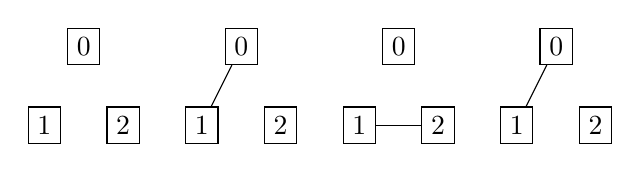
\begin{tikzpicture}
            \node[draw] (0) at (-11.5,1) {0};
            \node[draw] (1) at (-12,0) {1};
            \node[draw] (2) at (-11,0) {2};

            \node[draw] (0a) at (-9.5,1) {0};
            \node[draw] (1a) at (-10,0) {1};
            \node[draw] (2a) at (-9,0) {2};
            \draw (0a) -- (1a);

            \node[draw] (0b) at (-7.5,1) {0};
            \node[draw] (1b) at (-8,0) {1};
            \node[draw] (2b) at (-7,0) {2};
            \draw (1b) -- (2b);

            \node[draw] (0c) at (-5.5,1) {0};
            \node[draw] (1c) at (-6,0) {1};
            \node[draw] (2c) at (-5,0) {2};
            \draw (1c) -- (0c);

        \end{tikzpicture}
    \end{center}
    \begin{center}
        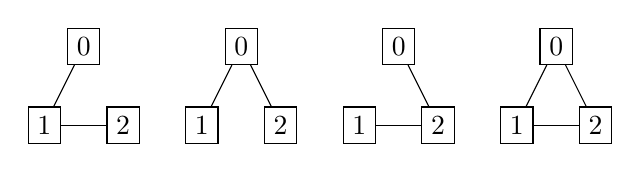
\begin{tikzpicture}
            
            \node[draw] (0d) at (-3.5,1) {0};
            \node[draw] (1d) at (-4,0) {1};
            \node[draw] (2d) at (-3,0) {2};
            \draw (1d) -- (0d);
            \draw (1d) -- (2d);

            \node[draw] (0e) at (-1.5,1) {0};
            \node[draw] (1e) at (-2,0) {1};
            \node[draw] (2e) at (-1,0) {2};
            \draw (1e) -- (0e);
            \draw (0e) -- (2e);

            \node[draw] (0f) at (0.5,1) {0};
            \node[draw] (1f) at (0,0) {1};
            \node[draw] (2f) at (1,0) {2};
            \draw (1f) -- (2f);
            \draw (0f) -- (2f);

            \node[draw] (0f) at (2.5,1) {0};
            \node[draw] (1f) at (2,0) {1};
            \node[draw] (2f) at (3,0) {2};
            \draw (1f) -- (0f);
            \draw (0f) -- (2f);
            \draw (1f) -- (2f);
        \end{tikzpicture}
    \end{center}
\end{frame}

\section{Exercice 2}
\begin{frame}
    \frametitle{Exercice 2}

    degrés:
    \begin{itemize}
        \item A: 4
        \item B: 2
        \item C: 2
        \item D: 3
        \item E: 2
        \item F: 1
    \end{itemize}
    $$\sum_{s\in S}{deg(s)}=14=2.A$$
\end{frame}
\begin{frame}[fragile]
    \frametitle{}

    \begin{enumerate}
        \item Matrice d'adjacence
              $$\begin{pmatrix}
                      0 & 1 & 1 & 1 & 0 & 1 \\
                      1 & 0 & 0 & 1 & 0 & 0 \\
                      1 & 0 & 0 & 0 & 1 & 0 \\
                      1 & 1 & 0 & 0 & 1 & 0 \\
                      0 & 0 & 1 & 1 & 0 & 0 \\
                      1 & 0 & 0 & 0 & 0 & 0 \\
                  \end{pmatrix}$$
        \item Dictionnaire d'adjacence
              \begin{lstlisting}[language=Python , basicstyle=\ttfamily\small, xleftmargin=2em, xrightmargin=2em]
g = {"A": ["B", "C", "D", "F"],
    "B": ["A", "D"],
    "C": ["A", "E"],
    "D": ["A", "B", "E"],
    "E": ["C", "D"],
    "F": ["A"]} 
\end{lstlisting}
    \end{enumerate}
\end{frame}
\section{Exercice 3}
\begin{frame}[fragile]
    \frametitle{Exercice 3}
Le graphe est complet.
    
\begin{center}
\begin{lstlisting}[language=Python , basicstyle=\ttfamily\small, xleftmargin=2em, xrightmargin=2em]
mat = [ [0, 1, 1, 1, 1],
        [1, 0, 1, 1, 1],
        [1, 1, 0, 1, 1],
        [1, 1, 1, 0, 1],
        [1, 1, 1, 1, 0]]
\end{lstlisting}
\captionof{code}{Matrice d'adjance}
\label{CODE}
\end{center}
\end{frame}
\begin{frame}[fragile]
    \frametitle{}

\begin{center}
\begin{lstlisting}[language=Python , basicstyle=\ttfamily\small, xleftmargin=2em, xrightmargin=2em]
def ordre(mat: list) -> int:
    return len(mat)
\end{lstlisting}
\end{center}    
\begin{center}
\begin{lstlisting}[language=Python , basicstyle=\ttfamily\small, xleftmargin=2em, xrightmargin=2em]
>>> ordre(mat)
5
\end{lstlisting}
\captionof{code}{Appel}
\label{CODE}
\end{center}
\end{frame}
\begin{frame}[fragile]
    \frametitle{}

\begin{center}
\begin{lstlisting}[language=Python , basicstyle=\ttfamily\small, xleftmargin=2em, xrightmargin=2em]
def est_complet(mat: list) -> bool:
    """
    vérifie si chaque sommet est relié à tous
    les autres (sauf lui même)
    """
    for ligne in range(ordre(mat)):
        for col in range(ordre(mat)):
            if ligne != col and mat[ligne][col] == 0:
                return False
    return True
\end{lstlisting}
\end{center}  
\begin{center}
\begin{lstlisting}[language=Python , basicstyle=\ttfamily\small, xleftmargin=2em, xrightmargin=2em]
>>> est_complet(mat)
True
\end{lstlisting}
\captionof{code}{Appel}
\label{CODE}
\end{center}
\end{frame}
\section{Exercice 4}
\begin{frame}[fragile]
    \frametitle{Exercice 4}


    \begin{itemize}
        \item 0: $d^+=2, d^-=0$
        \item 1: $d^+=1, d^-=0$
        \item 2: $d^+=1, d^-=1$
        \item 3: $d^+=0, d^-=3$
        \item 4: $d^+=1, d^-=2$
        \item 5: $d^+=1, d^-=2$
    \end{itemize}
    \begin{center}
\begin{lstlisting}[language=Python , basicstyle=\ttfamily\small, xleftmargin=1em, xrightmargin=0em]
suivants = [[3, 5], [3], [4], [], [3, 5], [2]]
\end{lstlisting}
\end{center}
\end{frame}
\begin{frame}[fragile]
    \frametitle{}

\begin{center}
\begin{lstlisting}[language=Python , basicstyle=\ttfamily\small, xleftmargin=1em, xrightmargin=0em]
def degres_sortants(liste: list, s: int) -> int:
    return len(liste[s])
\end{lstlisting}
\end{center}
\begin{center}
\begin{lstlisting}[language=Python , basicstyle=\ttfamily\small, xleftmargin=2em, xrightmargin=2em]
>>> degres_sortants(suivants, 4)
2
\end{lstlisting}
\captionof{code}{Appel}
\label{CODE}
\end{center}
\end{frame}
\begin{frame}[fragile]
    \frametitle{}

\begin{center}
\begin{lstlisting}[language=Python , basicstyle=\ttfamily\small, xleftmargin=1em, xrightmargin=0em]
def degres_entrants(liste: list, s: int) -> int:
    deg = 0
    for liste_successeurs in liste:
        for successeurs in liste_successeurs:
            if successeurs == s:
                deg = deg+1
    return deg
\end{lstlisting}
\end{center}
\begin{center}
\begin{lstlisting}[language=Python , basicstyle=\ttfamily\small, xleftmargin=2em, xrightmargin=2em]
>>> degres_entrants(suivants, 4)
1
\end{lstlisting}
\captionof{code}{Appel}
\label{CODE}
\end{center}
\end{frame}
\end{document}